% Chapter 6, changed from chapter 5 - still labelled as chapter 5

\chapter{Antigen Expression as a Determinant of CTL Lysis in HTLV-I Infection} % Write in your own chapter title
\label{Chapter5}
\lhead{Chapter 6. \emph{Antigen Expression as a Determinant of CTL Lysis}}

\section{Introduction}

So far, this study has concentrated on the epitope properties that are associated with disease risk and proviral load. For this chapter, we extended this work to examine the CD8$^+$ T cell response itself, specifically in terms of its dynamics as a function of antigen expression of infected CD4$^+$ T cells. 

In human T-lymphotropic virus type 1 (HTLV-I) infection, a high frequency of HTLV-I-specific CTLs can co-exist stably with a high
proviral load and the proviral load is strongly correlated with the risk of HTLV-I-associated inflammatory diseases. In \cref{Chapter2}, \sref{chapter2/CTLResponse}, it was discussed how these observations have led to the hypothesis that HTLV-I specific CTLs are ineffective in controlling HTLV-I replication but contribute to the pathogenesis of the inflammatory diseases. However, evidence from host and viral immunogenetics and gene expression microarrays suggests that a strong CTL response is associated with a low proviral load and a low risk of HAM/TSP. To further examine the role of CTLs in HTLV-I infection, a collaborative experiment was carried out to quantify the frequency, lytic activity and functional avidity of HTLV-I-specific CD8$^+$ cells in fresh, unstimulated PBMCs from individuals with natural HTLV-I infection. The ELISpot assays and flow cytometry experiments were performed by Aileen Rowan and Tarek Kattan. My role, using a system of ordinary differential equations, was to quantify the efficiency of CD8$^+$ lysis in their \emph{ex vivo} experiments.   

We have previously investigated methods of quantifying antiviral CTL efficiency. In HTLV-I infection, both effector CTLs and infected target cells are often present in fresh blood at frequencies sufficiently high to obviate the need for enrichment of specific
subpopulations. We have exploited this feature to develop an assay of CD8$^+$ cell-mediated suppression of HTLV-I expression in
fresh PBMCs \citep{Asquith2005a}. As a marker of proviral expression we use the viral protein Tax, a regulatory protein expressed early in the life cycle of HTLV-I \citep{Asquith2005a}. We previously showed that this suppression of HTLV-I depended on CD8$^+$ T cell frequency and required both perforin and a match in class 1 MHC genotype between effector and target cells \citep{Hanon2000}, consistent with classical class 1 MHC-restricted CTL lysis. Mathematical modeling can be used to quantify the rate of killing of Tax-expressing CD4$^+$ cells per CD8$^+$ cell per day. We use the term lytic efficiency to denote this per-CD8$^+$-cell rate of lysis. This assay of lytic efficiency showed that the rate of CTL-mediated lysis of HTLV-I-infected cells in fresh PBMCs was inversely correlated with the proviral load, both in patients with HAM/TSP and in asymptomatic HTLV-I carriers (ACs) \citep{Asquith2005a}.

This measure of lytic efficiency has two chief limitations. First, the antiviral activity is expressed per CD8$^+$ cell, not per virus-specific CD8$^+$ cell, since there is no currently available method to measure in the same assay the lytic activity and the total frequency of CD8$^+$ T cells specific to all viral epitopes in each individual (an ELISpot assay that detects IFN$\gamma$ production comes closest to this definition. However, this assay only detects the activation of CD8$^+$ cells and not their lytic efficiency). Second, rate of lysis is likely to be a composite parameter that is a function of both the frequency of the Ag specific CD8$^+$ cells and the ``quality'' of their effector functions at the single-cell level \citep{Seder2008} (i.e.~it is not clear what effector functions might affect the lysis rate). In an acute viral infection, efficient elimination of the virus is associated with a high frequency of Ag-specific T cells \citep{Stambas2007}. But in persistent infections, the complexity of the equilibrium dynamics makes it impossible to infer the efficiency of virus-specific CTLs directly from their steady-state frequency \citep{Asquith2007}.

For this chapter, I modified this model of lytic efficiency to take account of the observation that Tax expression per cell is not constant in the HTLV-I-infected target CD4$^+$ cells, but increases over the 18 hour incubation time. The results of this analysis were estimates of the lytic efficiency of CTLs specific to high Tax expressing cells and, separately, low Tax expressing cells.

%%%%%%%%%%%%%%%%%%%%%%%%%%%%%%%%%%%%%%%%%%%%%%%%%%%%%%%%%%%%%%%%%%%%%%%%%%%%%%%%%%%%%%%%%%%%%%%%%%%%

\section{Methods}

The cell preparation, culture and flow cytometry analysis was carried out by Tarek Kattan.

\subsection{PBMC Separation}

Peripheral blood mononuclear cells (PBMCs) were isolated from whole blood by density gradient centrifugation using Histopaque-1077 (Sigma, Poole, United Kingdom) from EDTA-anticoagulated blood samples taken from HTLV-I infected individuals. All individuals attended the HTLV-I clinic at St Mary�s Hospital, London and gave written informed consent. Isolated PBMCs were washed twice in PBS and then cryopreserved in fetal calf serum (FCS, Sigma) with 10\% dimethyl sulfoxide (DMSO, Sigma).

\subsection{Cell Culture}\label{chapter5/methodsCulture}

Cells were thawed, washed twice in PBS and then cultured in complete medium consisting of RPMI 1640 medium (Sigma) supplemented with
10\% FCS, 2 mM L-Glutamine, 100 U/ml Penicillin and 100$\mu$g/ml Streptomycin (Life Technologies). Cells were incubated for different times at $37\,^{\circ}\mathrm{C}$ in 5\% CO$_2$. When required, CD8$^+$ or CD4$^+$ cells were depleted by positive selection using Ab coated magnetic microbeads following the manufacturer's instructions (Miltenyi Biotec, Surrey, United Kingdom).

\subsection{Flow Cytometric Detection of Tax Expression}

After incubation, cells were surface-stained with mAbs specific to CD4 and CD8 at 15$\mu$g/ml in each case (Beckman Coulter, Marseille, France). Cells were fixed with 2\% paraformaldehyde (PFA, Sigma) and then permeabilized using PBS/0.1\% Triton X-100 (Sigma). Finally, cells were stained intracellularly with the FITC conjugated Ab anti-Tax protein Lt-4 \citep{Lee1989}, diluted 1/100. Cells were analyzed on a Coulter Epics XL flow cytometer. Thirty thousand events were routinely collected during acquisition of the data. The data were analyzed using Coulter Expo32 software (Beckman Coulter). Tax$^+$cells were divided in flow-cytometric analysis into two gates, corresponding respectively to Tax\superscript{low} and Tax\superscript{high} cells according to fluorescence intensity. The line dividing these gates was arbitrarily defined; the same definition was used in the analysis of all samples.

\subsection{Rate of CD8$^+$ Cell-mediated Lysis}\label{chapter5/methodsLysis}

The rate (``efficiency'') of CD8$^+$ cell-mediated lysis of HTLV-I-infected cells was estimated as previously described \citep{Asquith2005a}. CD8$^+$ cell lytic efficiency (expressed as the proportion of Tax-expressing CD4$^+$ cells killed per CD8$^+$ cell per day) was calculated for each HTLV-I-infected individual tested using \eref{chapter5/equation1}:

\begin{equation}
\frac{dy}{dt} = c - \epsilon y z
\label{chapter5/equation1}
\end{equation}

where $y$ is the proportion of CD4$^+$ cells expressing Tax, $c$ is the rate of increase of Tax expression, which is assumed to be constant during the short-term culture, $\epsilon$ is the CD8$^+$ cell-mediated antiviral efficacy (expressed as the proportion of CD4$^+$ Tax$^+$ cells killed per CD8$^+$ cell per day) and $z$ is the proportion of lymphocytes that are CD8$^+$. This model was solved analytically and fitted to the data using non-linear least-squares regression (SPSS v12), providing an estimate of the antiviral efficacy ($\epsilon$) in each individual.

\eref{chapter5/equation1} used a constant rate $c$ to describe Tax expression in the absence of CD8$^+$ cells. However, since observations from experimental time course data (\fref{chapter5/figureTimeCourse}) suggested a non-linear rate of increase of Tax expression, it was necessary to modify the existing model. 2 models were considered as possibilities:

\begin{center}

\begin{tikzpicture}[nonterminal/.style={
	rectangle,
	minimum size=12mm,
	very thick,
	draw=red!50!black!50, 
	top color=white, 
	bottom color=red!50!black!20,
	font=\itshape
	},terminal/.style={
	rectangle,minimum size=6mm,rounded corners=3mm,
	very thick,draw=black!50,
	top color=white,bottom color=black!20,
	font=\ttfamily
	}
]

\node (atom1) [nonterminal] {Tax Negative};
\node (rate1) [terminal,right=of atom1] {C$_1$};
\node (atom2) [nonterminal,right=of rate1] {Tax Low};
\node (rate2) [terminal,right=of atom2] {C$_2$};
\node (atom3) [nonterminal,right=of rate2] {Tax High};

\path	(atom1) edge[-] (rate1)
	(rate1) edge[->] (atom2)
	(atom2) edge[-] (rate2)
	(rate2) edge[->] (atom3);

\node (atom4) [nonterminal, below=of atom1, yshift=-20mm] {Tax Negative};
\node (rate3) [terminal, above right=of atom4, yshift=-10mm] {C$_1$};
\node (rate4) [terminal, below right=of atom4, yshift=10mm] {C$_2$};
\node (atom5) [nonterminal, right=of rate3, yshift=8mm] {Tax Low};
\node (atom6) [nonterminal, right=of rate4, yshift=-8mm] {Tax High};

\path	(atom4) edge[-] (rate3)
	(rate3) edge[->] (atom5)
	(atom4) edge[-] (rate4)
	(rate4) edge[->] (atom6);

\end{tikzpicture}
\end{center}

The first model represents a progression from Tax\superscript{negative} to Tax\superscript{low} to Tax\superscript{high} expressing CD4$^+$ cells as a single population. The second models the appearance of Tax\superscript{low} and Tax\superscript{high} expressing CD4$^+$ cells as 2 distinct populations. Instead of a single parameter $c$ that defines the rate of increase of Tax expression in \eref{chapter5/equation1}, each model introduces 2 rate parameters: $c_1$, the rate of increase of low Tax expression and $c_2$, the rate of increase of high Tax expression. Both models were fitted to the time course data and it was found that the `single population' model was a more accurate fit of the data (see \sref{chapter5/results/TaxExpress}). The `single population' model was designated `Model 1'.

In Model 1, the Tax\superscript{low} population (as defined from the gated FACS) is produced at a constant rate $c_1$ and the Tax\superscript{high} population at a rate $c_2$. The following pair of linked ordinary differential equations, \eref{chapter5/equation2} and \eref{chapter5/equation3}, describe the model:

\begin{equation}
\frac{dy}{dt} = c_1 - c_2y
\label{chapter5/equation2}
\end{equation}

\begin{equation}
\frac{dw}{dt} = c_{2}y
\label{chapter5/equation3}
\end{equation}

Here, $y$ is the proportion of CD4$^+$ cells expressing low levels of Tax and $w$ is the proportion of CD4$^+$ cells expressing high levels of Tax. Solving these equations, we have \eref{chapter5/equation4} and \eref{chapter5/equation5}:

\begin{equation}
y = \left( \frac{c_1}{c_2} \right) \left( 1 - e^{-c_2 t} \right)
\label{chapter5/equation4}
\end{equation}

\begin{equation}
w = c_1 \left( t + \frac{e^{-c_2 t}}{c_2} - \frac{1}{c_2} \right)
\label{chapter5/equation5}
\end{equation}

\eref{chapter5/equation4} and \eref{chapter5/equation5} were fitted to the data using non-linear least-squares regression (\tref{chapter5/table1}), providing an estimate for $c_1$ and $c_2$ in each individual. \eref{chapter5/equation2} and \eref{chapter5/equation3} were then modified to describe the rate of CD8$^+$ cell-mediated lysis of Tax\superscript{low} CD4$^+$ cells and Tax\superscript{high} CD4$^+$ cells separately:

\begin{equation}
\frac{dy}{dt} = c_1 - c_2 y - \epsilon^{\text{low}} y z 
\label{chapter5/equation6}
\end{equation}

\begin{equation}
\frac{dw}{dt} = c_1\left(1 - \frac{1}{e^{c_2t}}\right) - \epsilon^{\text{high}} w z 
\label{chapter5/equation7}
\end{equation}

\eref{chapter5/equation6} and \eref{chapter5/equation7} (Model 2) were solved analytically and fitted to the data using non-linear least-squares regression. From the resulting data, estimates for the rate of killing of CD4$^+$ cells expressing low levels of Tax ($\epsilon$\superscript{low}) and high levels of Tax ($\epsilon$\superscript{high}) were produced for each individual.

\subsubsection{Bootstrap}\label{chapter5/methodsBootstrap}

A bootstapping method was used to test the robustness of the $\epsilon$\superscript{low} and $\epsilon$\superscript{high} parameters for each patient. 50 new datasets were generated per individual for both their expression levels of Tax\superscript{low} and Tax\superscript{high}. \eref{chapter5/equation6} and \eref{chapter5/equation7} were then fitted to this data, which gave a standard deviation of the resulting values of $\epsilon$\superscript{low} and $\epsilon$\superscript{high} (see \tref{chapter5/table1}).

%%%%%%%%%%%%%%%%%%%%%%%%%%%%%%%%%%%%%%%%%%%%%%%%%%%%%%%%%%%%%%%%%%%%%%%%%%%%%%%%%%%%%%%%%%%%%%%%%%%%

\section{Results}

\subsection{Modeling Tax expression}\label{chapter5/results/TaxExpress}

Flow cytometric analysis was used to divide the Tax-expressing CD4$^+$ population into high Tax-expressing and low Tax-expressing
cells. The 2 models of Tax expression, `single' and `dual' populations, were solved and fitted to the experimental data to give estimates of the parameters $c_1$ and $c_2$ in each case. \tref{chapter5/tableTaxFits} shows the $R^2$ values for the fits of the respective models for each of the patients. The accuracy of the `single population' model was significantly better for low Tax expression and better for high Tax expression (Tax low: $P = 0.0001$, Tax high, $P = 0.095$; paired Wilcoxon-Mann-Whitney). From these results, we chose the `single population' as our model of Tax expression over 18 hours.

\begin{table}[htp]
\begin{center}

\begin{tabular}{|c|c|c|c|c|c|}
\hline
& Names & Single Low & Single High & Dual Low & Dual High \bigstrut \\
\hline
1 & HAP  & 0.4571 & 0.8297 & 0.1126 & 0.8575 \bigstrut[t] \\
2 & HAY  & 0.8710 & 0.8408 & 0.8586 & 0.1214 \\
3 & HBE  & 0.2665 & 0.4938 & -0.2782 & 0.4277 \\
4 & HBX  & 0.7376 & -1.4986 & 0.6609 & 0.2523 \\
6 & HCH  & 0.1675 & 0.4303 & -0.2767 & 0.7503 \\
8 & HFB  & -1.0925 & 0.7753 & -2.6407 & 0.7978 \\
11 &  TAK & 0.8165 & 0.4660 & 0.8179 & 0.0435 \\
12 &  TAQ & 0.9461 & 0.8541 & 0.9361 & 0.7629 \\
13 &  TAW & -0.0586 & -0.2140 & -0.5068 & 0.4870 \\
14 &  TAZ & 0.8401 & 0.7504 & 0.8006 & 0.0256 \\
15 &  TBC & 0.6124 & 0.9268 & -0.2076 & -0.7341 \\
16 &  TBJ & 0.7501 & 0.6986 & 0.5346 & -0.0517 \\
17 &  TBP & 0.7397 & 0.9457 & 0.3094 & -0.1896 \\
19 &  TCL & 0.6367 & 0.5781 & 0.3577 & 0.1122 \\
20 &  UV1 & -0.1119 & 0.6705 & -0.7201 & -1.6188 \bigstrut[b] \\
\hline
\end{tabular}
\end{center}

\caption[The accuaracy of alternative models of Tax expression]{The $R^2$ values showing the accuracy of the single and dual population models fitting the experimental time course data of Tax\superscript{low} and Tax\superscript{high} expression.}
\label{chapter5/tableTaxFits}
\end{table}

\eref{chapter5/equation2} and \eref{chapter5/equation3} were then fitted to the Tax\superscript{low} and Tax\superscript{high} data respectively by non-linear least squares regression. Values for the parameters $c_1$ and $c_2$ were calculated from this analysis for each of the 15 patients (\tref{chapter5/table1}). Examples for 6 of the patients are shown in \fref{chapter5/figureTimeCourse}. The data for the other 9 patients is in \aref{AppendixB}, \fref{appendixb/figureTimecourse}.


\begin{figure}[htp]
\centering
\includegraphics[width=7cm]{./Figures/chapter5/figure_timecourse_hap}%
\hspace{0cm}%
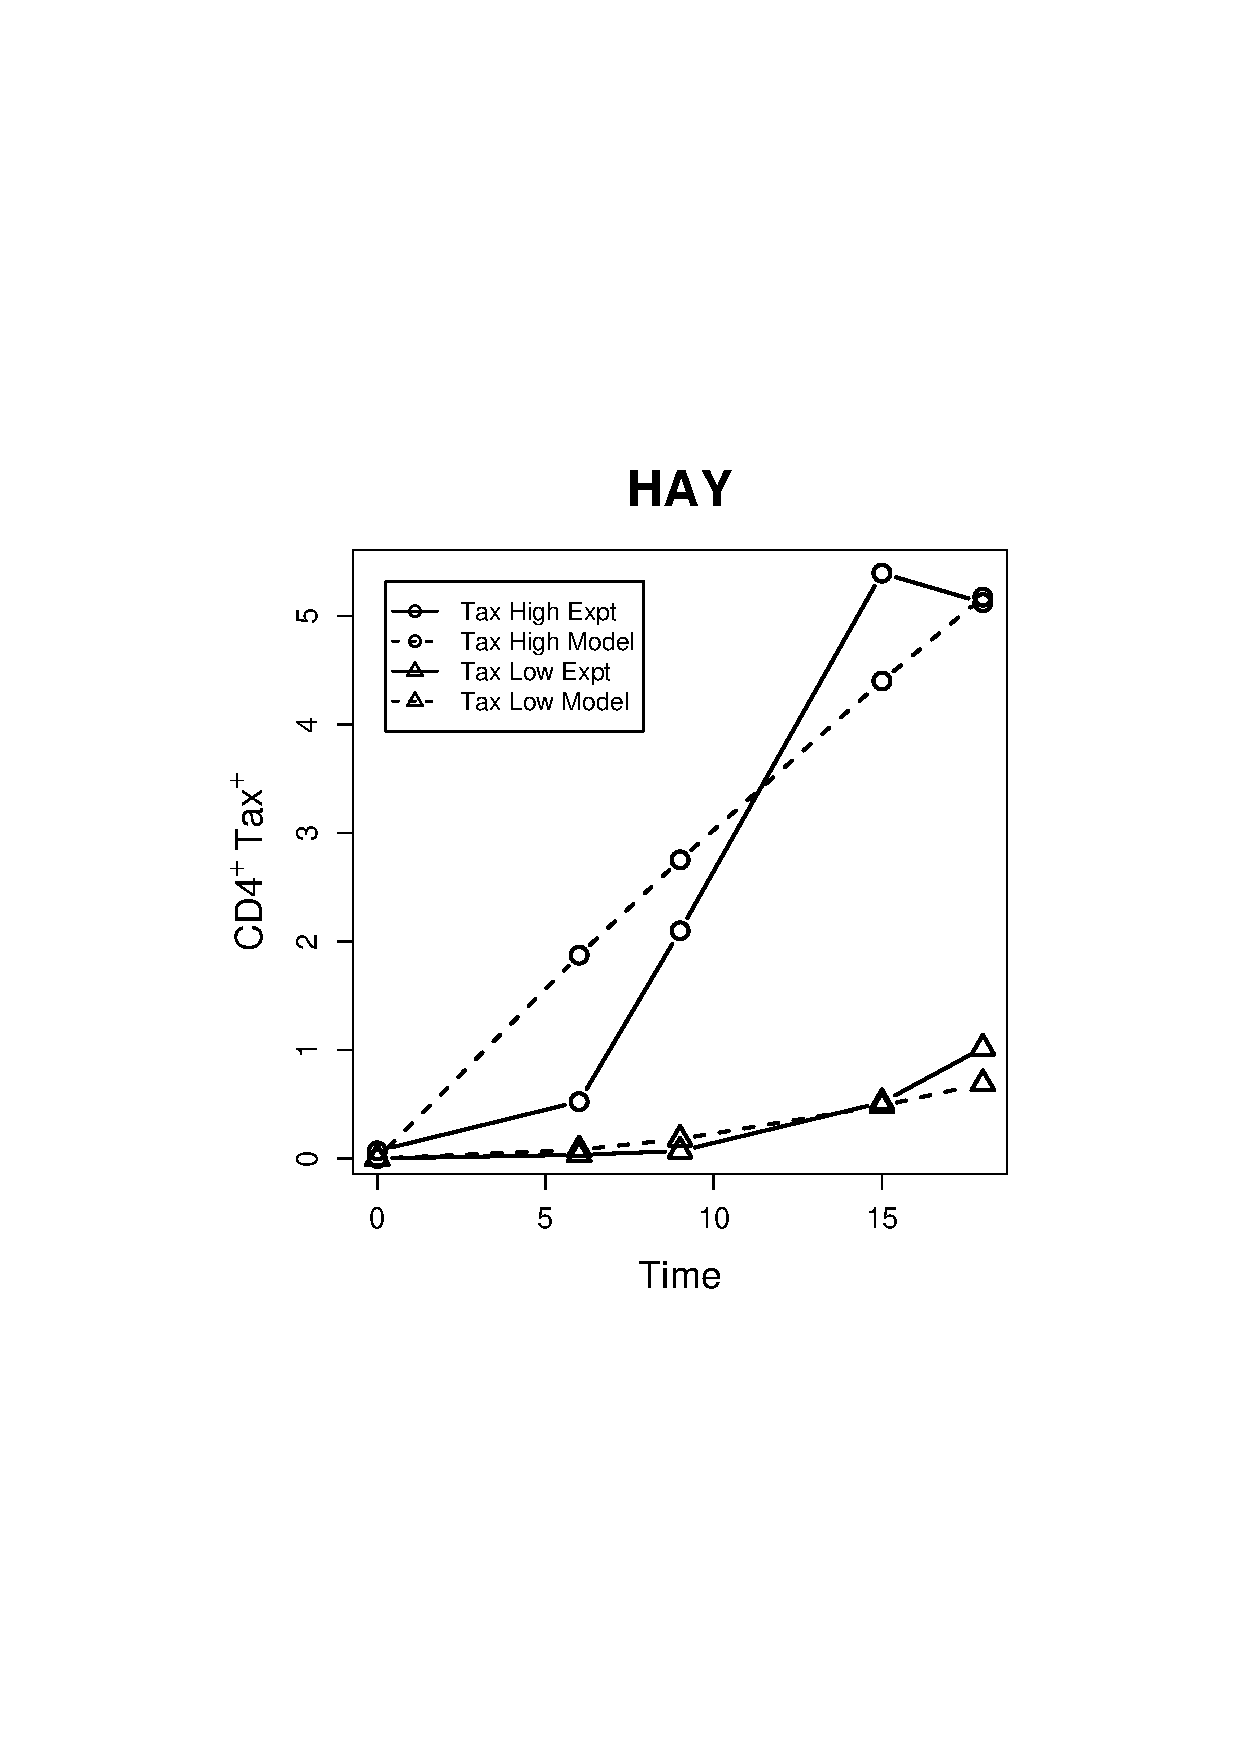
\includegraphics[width=7cm]{./Figures/chapter5/figure_timecourse_hay} \\
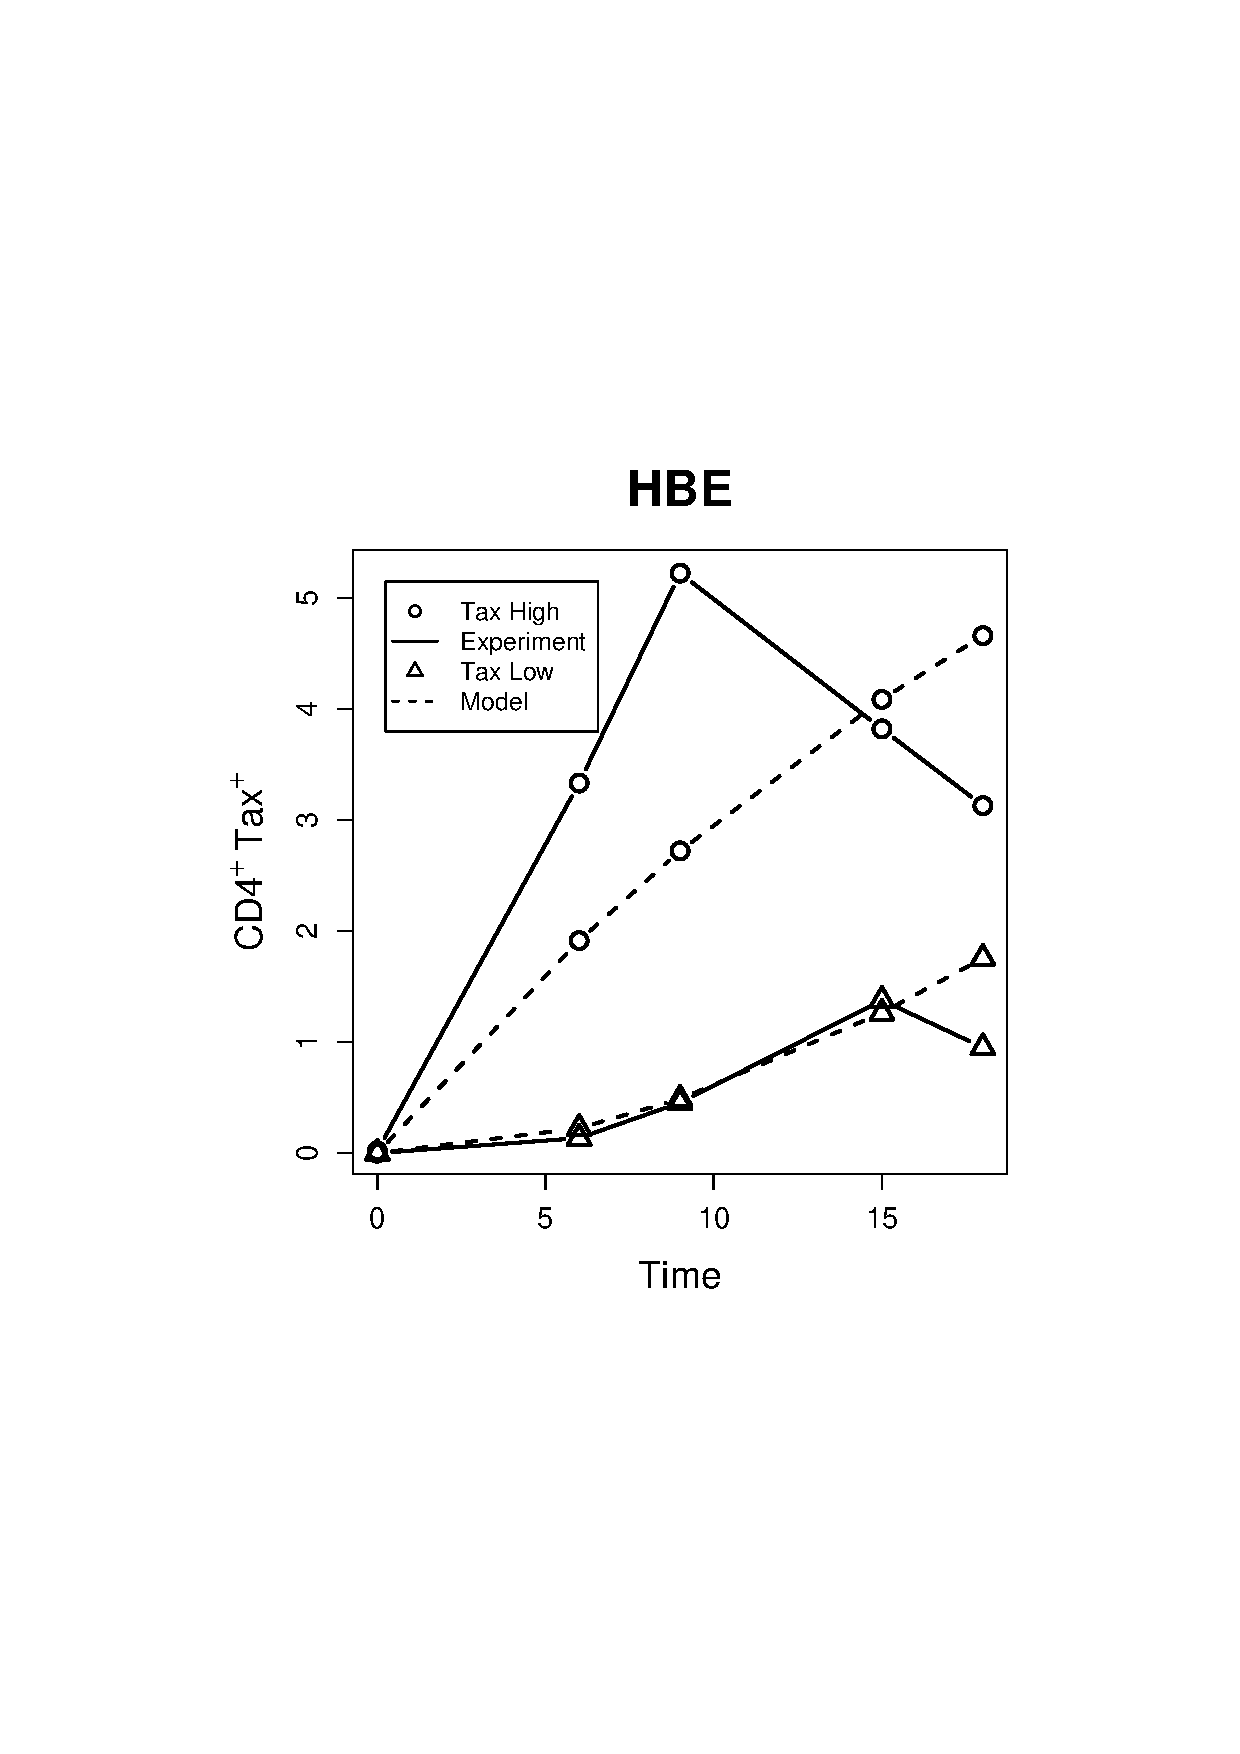
\includegraphics[width=7cm]{./Figures/chapter5/figure_timecourse_hbe}%
\hspace{0cm}%
\includegraphics[width=7cm]{./Figures/chapter5/figure_timecourse_hbx} \\
\includegraphics[width=7cm]{./Figures/chapter5/figure_timecourse_hch}%
\hspace{0cm}%
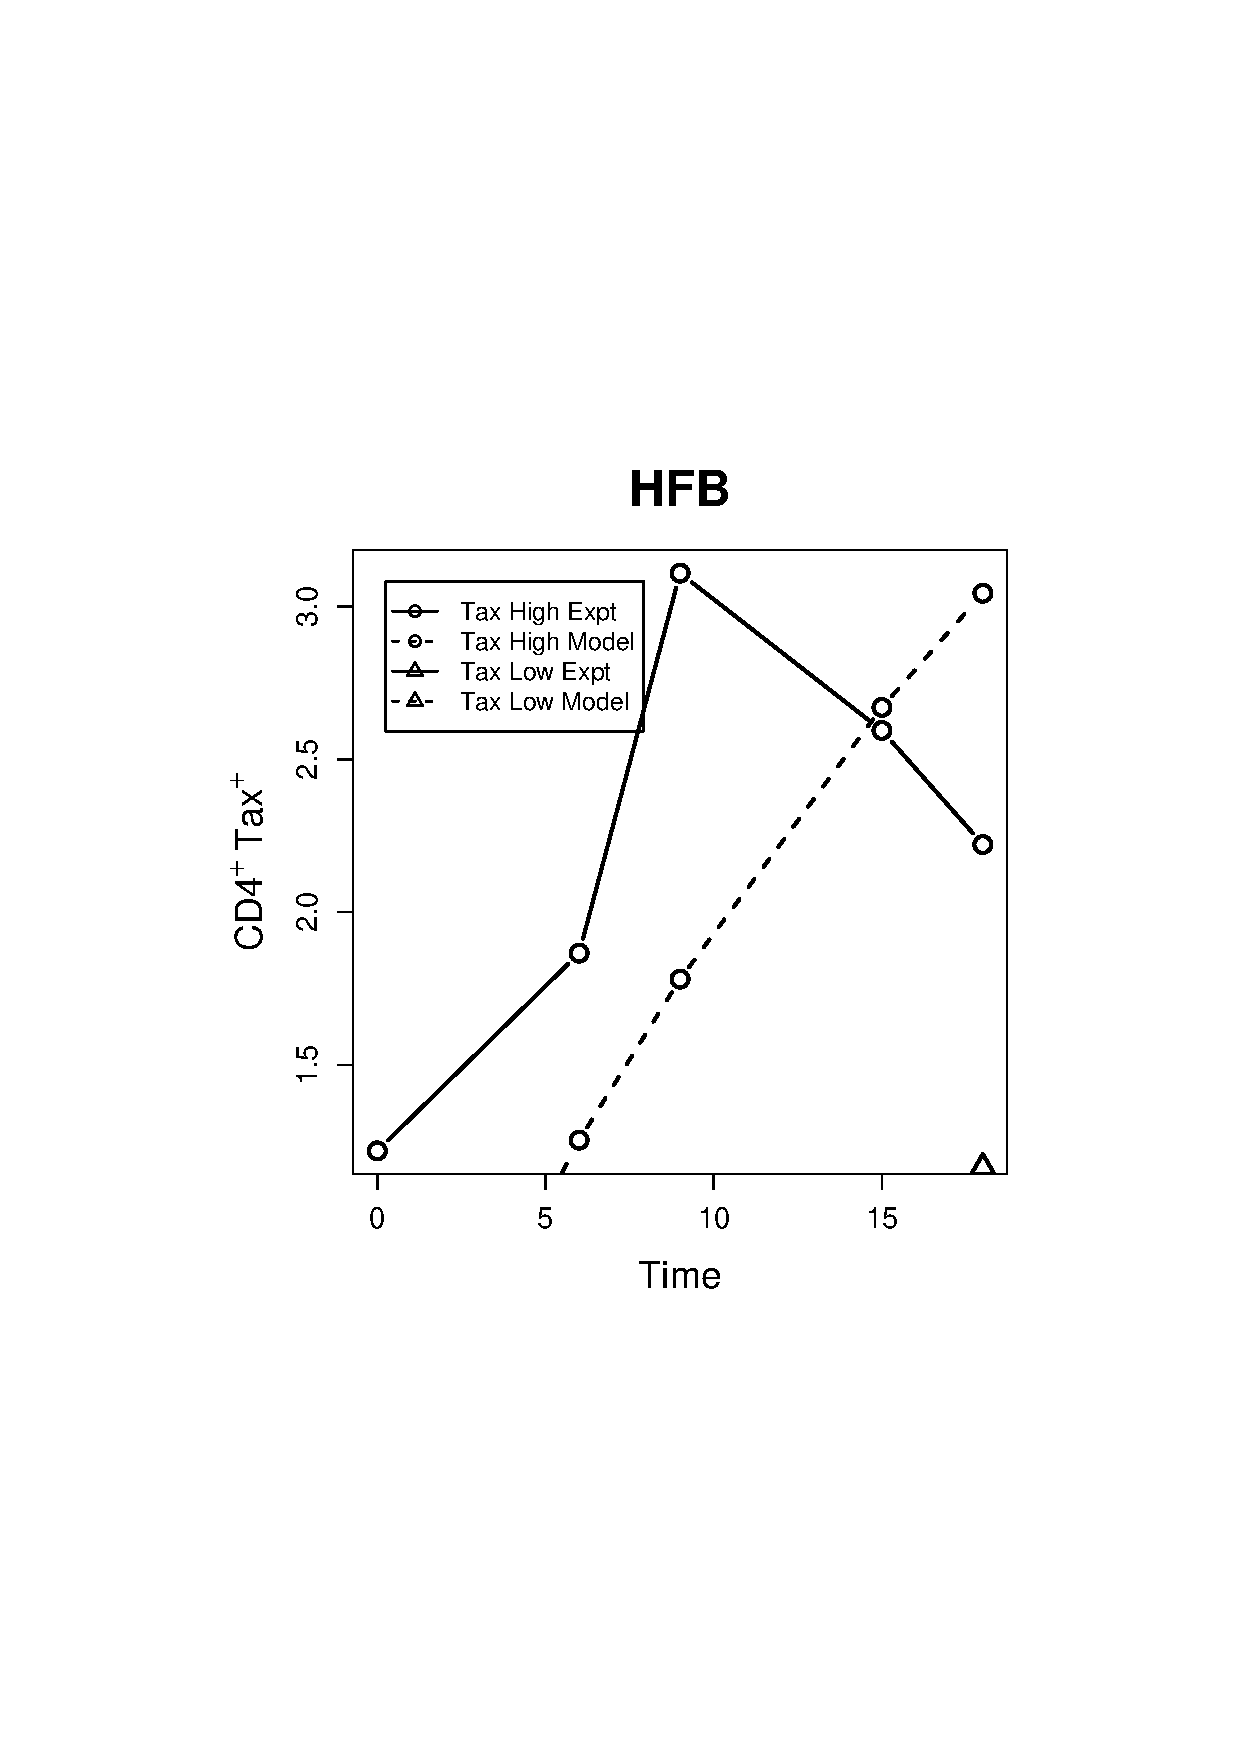
\includegraphics[width=7cm]{./Figures/chapter5/figure_timecourse_hfb} \\
\caption[The Tax expression time course]{This figure shows examples of the time course of Tax expression as the proportion of CD4$^+$ lymphocytes that were Tax\superscript{high} or Tax\superscript{low} over 18 hours culture (see \sref{chapter5/methodsCulture}). \eref{chapter5/equation2} and \eref{chapter5/equation3} were fitted to the Tax\superscript{low} and Tax\superscript{high} data respectively.}
\label{chapter5/figureTimeCourse}
\end{figure}

\subsection{The CD8$^+$ Antiviral Efficacy Assay}

\eref{chapter5/equation6} and \eref{chapter5/equation7} were fitted to the antiviral efficacy assay data for all 15 patients. The data shown for each patient is the proportion of CD4$^+$ lymphocytes that were Tax\superscript{high} and Tax\superscript{low} following 18 h co-culture with different proportions of CD8$^+$ lymphocytes. The parameters $\epsilon$\superscript{low} and $\epsilon$\superscript{high} were measured by non-linear least squares regression. The assay was repeated in each patient. \fref{chapter5/figureLysisAssay} shows this data for 3 patients. The data for the other 12 patients is in \aref{AppendixB}, \fref{appendixb/figureLysisHighLow}.

\fref{chapter5/figurePairedEpsilon} shows a statistically significantly higher rate of CD8$^+$ cell-mediated lysis of the Tax\superscript{high} cells than that of the Tax\superscript{low} cells ($P = 0.004$, Wilcoxon-Mann-Whitney, $n=15$). \fref{chapter5/figureCompareLysis} shows the plot of $\epsilon$\superscript{low} against $\epsilon$\superscript{high} for each patient. The strong linear relationship ($R^2 = 0.855$, $P < 0.001$) suggests the ratio $\epsilon$\superscript{high}/$\epsilon$\superscript{low} is maintained across patients.

There was strong agreememt between the 2 repeats per patients of the estimates for $\epsilon$\superscript{low} and $\epsilon$\superscript{high} ($\epsilon$\superscript{low}: $R^2 = 0.9492$, $P < 0.001$. $\epsilon$\superscript{high}: $R^2 = 0.890$, $P < 0.001$; \aref{AppendixB}, \fref{appendixb/figureLysisHighLow}). \aref{AppendixB} also contains a comparison of the original $\epsilon$ and $c$ parameters from \eref{chapter5/equation1} against $\epsilon$\superscript{low} and $\epsilon$\superscript{high} (\fref{appendixb/figure2}) and $c_1$ and $c_2$ (\fref{appendixb/figure3}).

Finally, \aref{AppendixB}, \fref{chapter5/figureRatio} shows there was no difference in the ratio of Tax expression between HAM/TSP patients and ACs ($P = 0.871$, Wilcoxon-Mann-Whitney, HAM/TSP: $n=16$, AC: $n=12$).

\begin{figure}[htp]
\centering
\includegraphics[width=7cm]{./Figures/chapter5/figure_lysis_hap_rep_1}%
\hspace{0cm}%
\includegraphics[width=7cm]{./Figures/chapter5/figure_lysis_hap_rep_2} \\
\includegraphics[width=7cm]{./Figures/chapter5/figure_lysis_hay_rep_1}%
\hspace{0cm}%
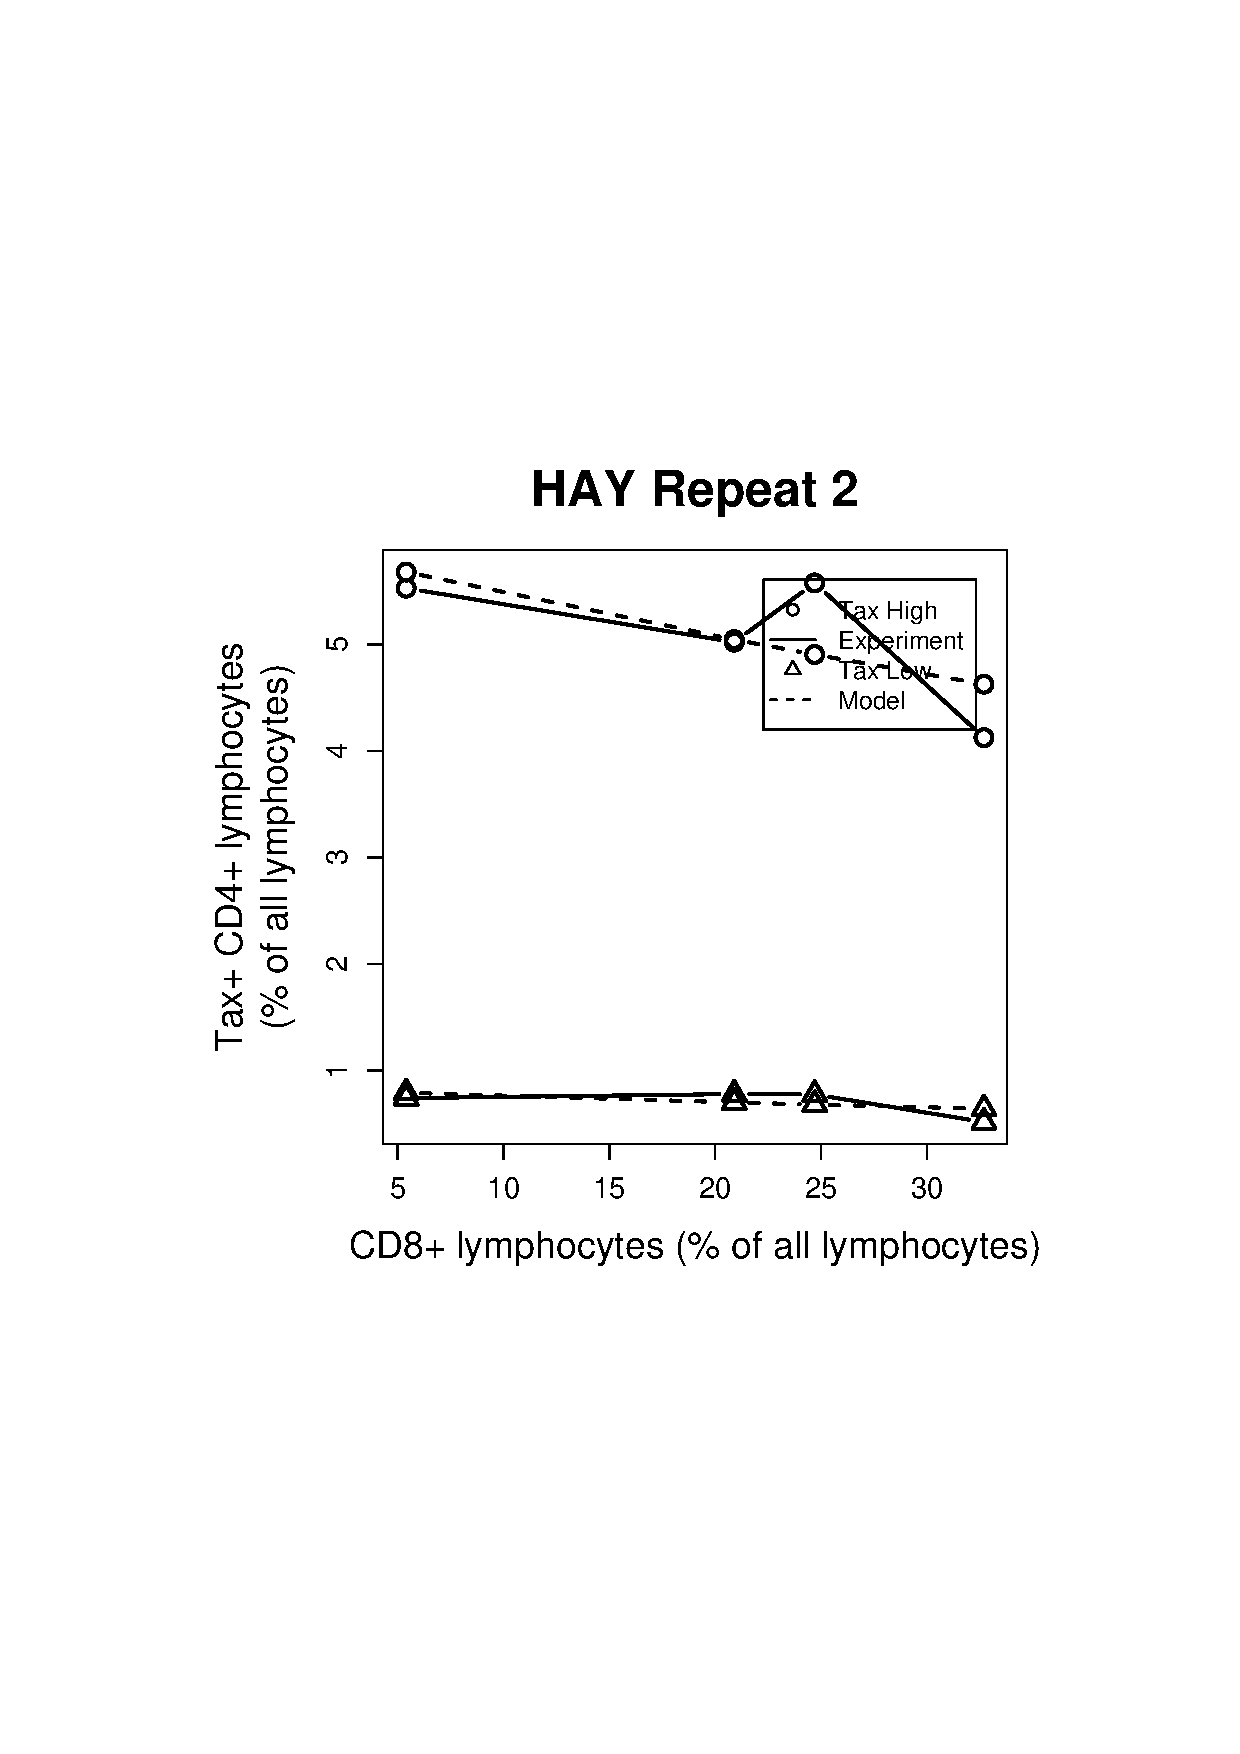
\includegraphics[width=7cm]{./Figures/chapter5/figure_lysis_hay_rep_2} \\
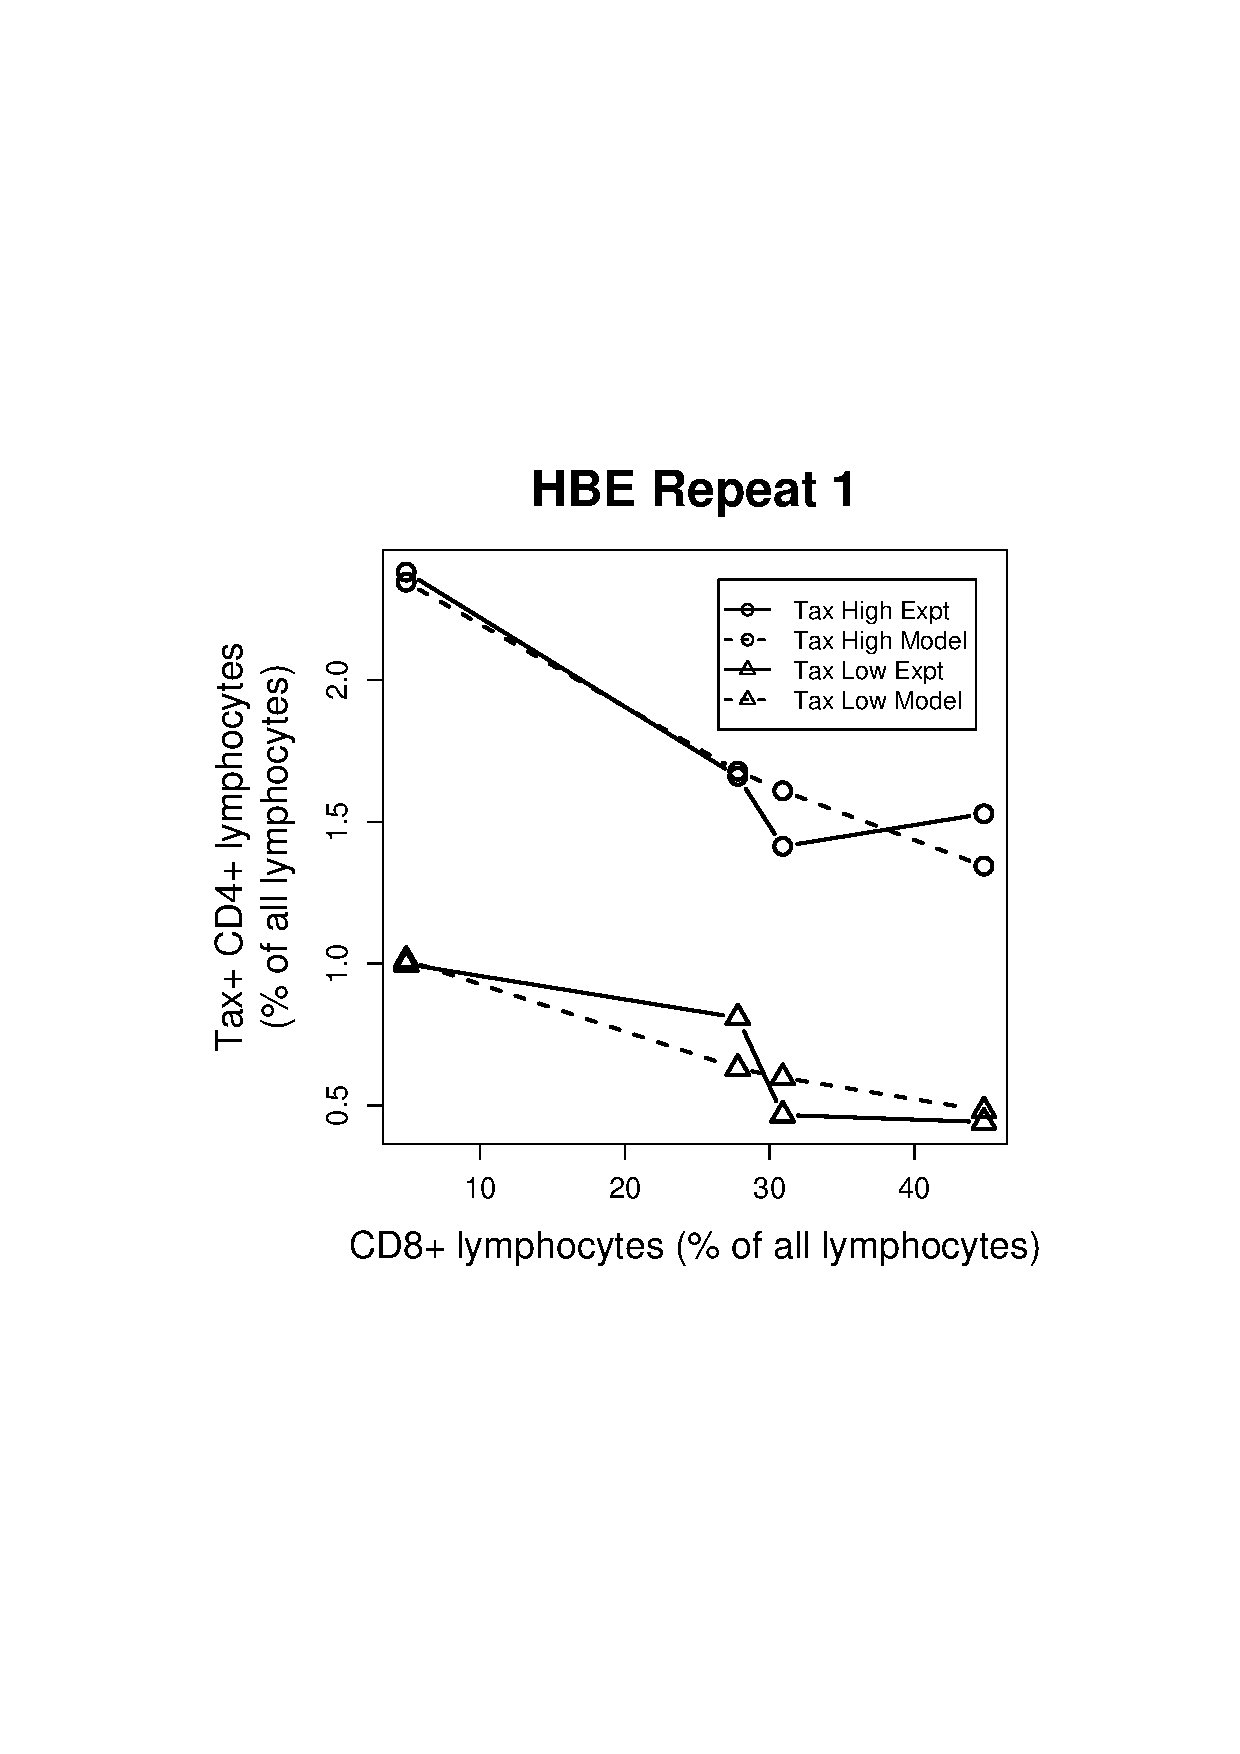
\includegraphics[width=7cm]{./Figures/chapter5/figure_lysis_hbe_rep_1}%
\hspace{0cm}%
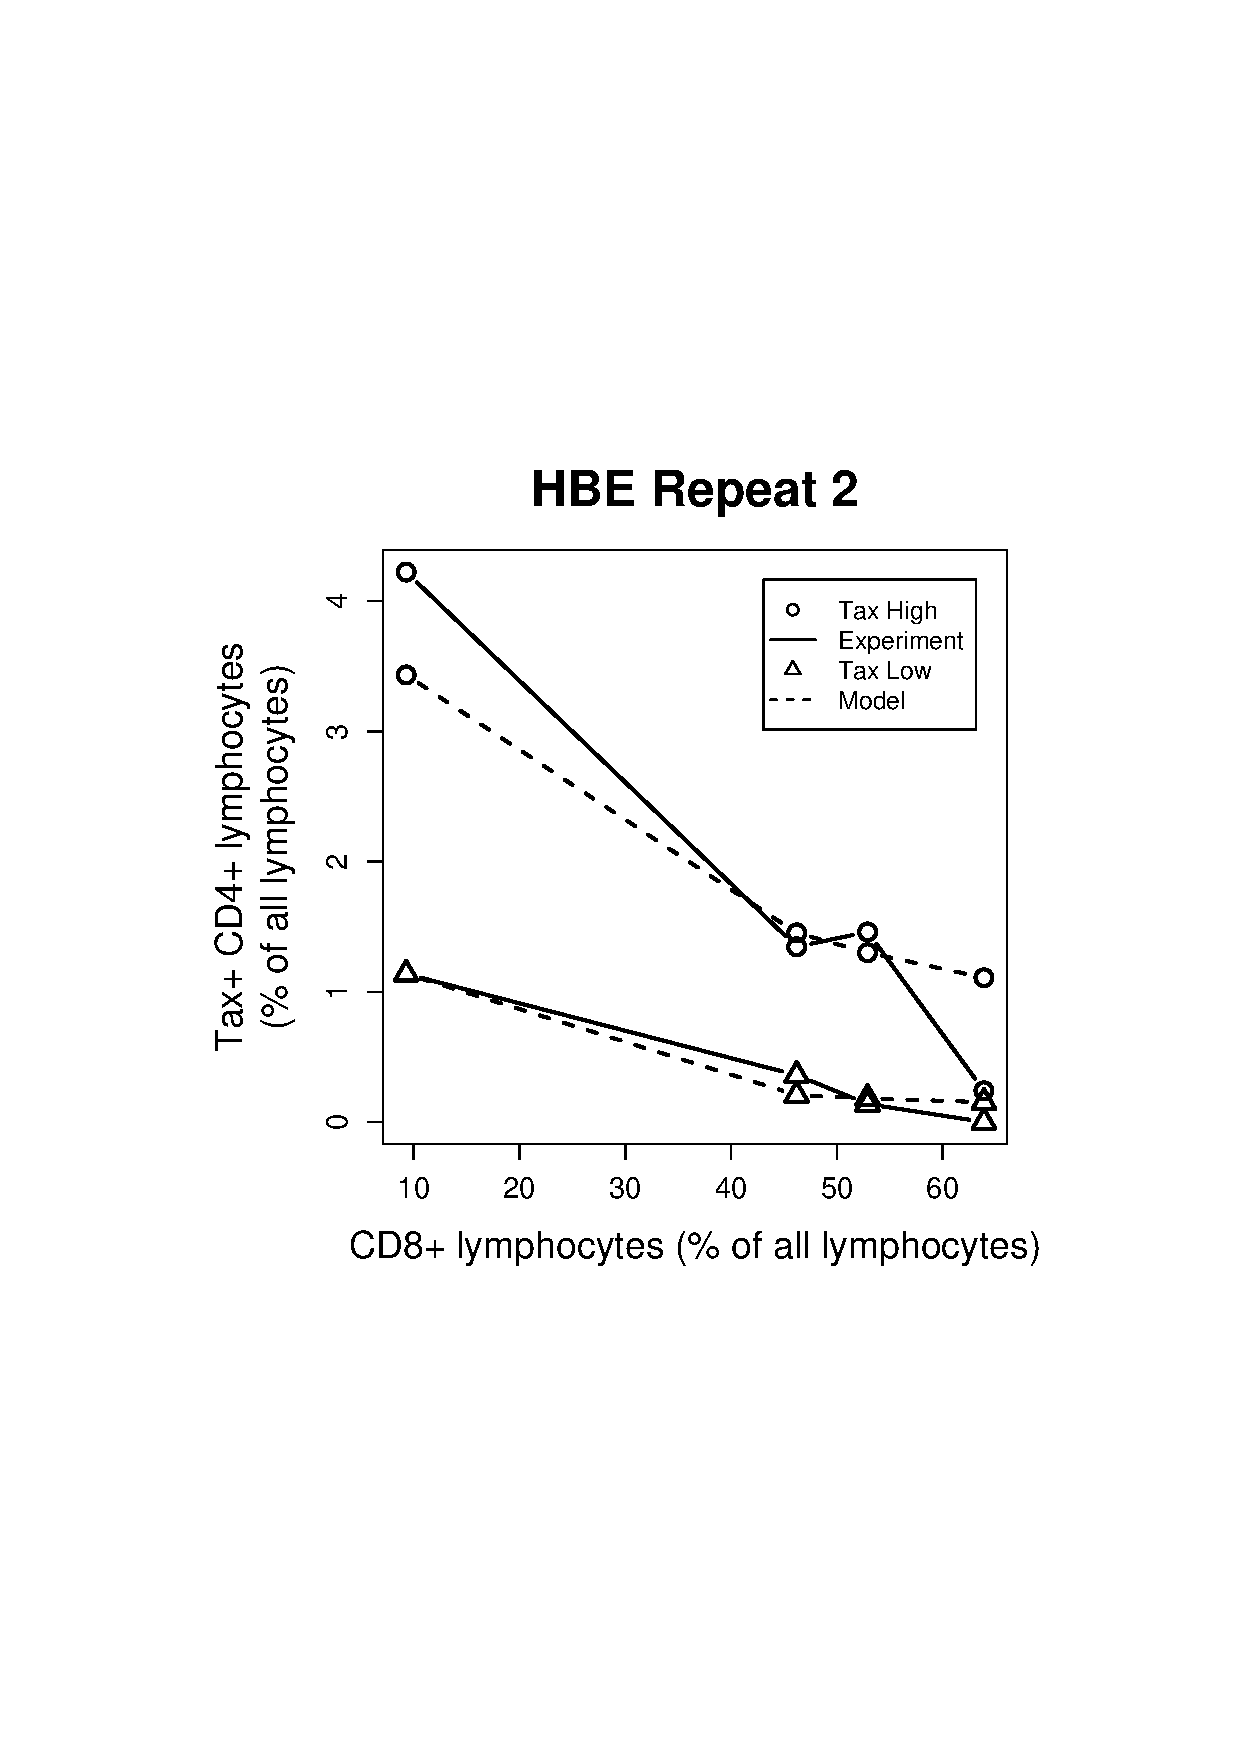
\includegraphics[width=7cm]{./Figures/chapter5/figure_lysis_hbe_rep_2} \\
\caption[CD8$^+$ antiviral efficacy assay]{The figure
shows examples of the antiviral efficacy assay for patients HAP, HAY and HBE. The proportion of CD4$^+$ lymphocytes that were Tax\superscript{high} and Tax\superscript{low} following 18 h co-culture with different proportions of CD8$^+$ lymphocytes was measured. The model (\eref{chapter5/equation6} and \eref{chapter5/equation7}, \sref{chapter5/methodsLysis}) was fitted to this data and in this way the rate of clearance of Tax\superscript{low}CD4$^+$ and Tax\superscript{high}CD4$^+$ cells per day per CD8$^+$ cell (antiviral efficacy) was estimated. This was repeated in the same subject.}
\label{chapter5/figureLysisAssay}
\end{figure}

\begin{figure}[htp]
\centering
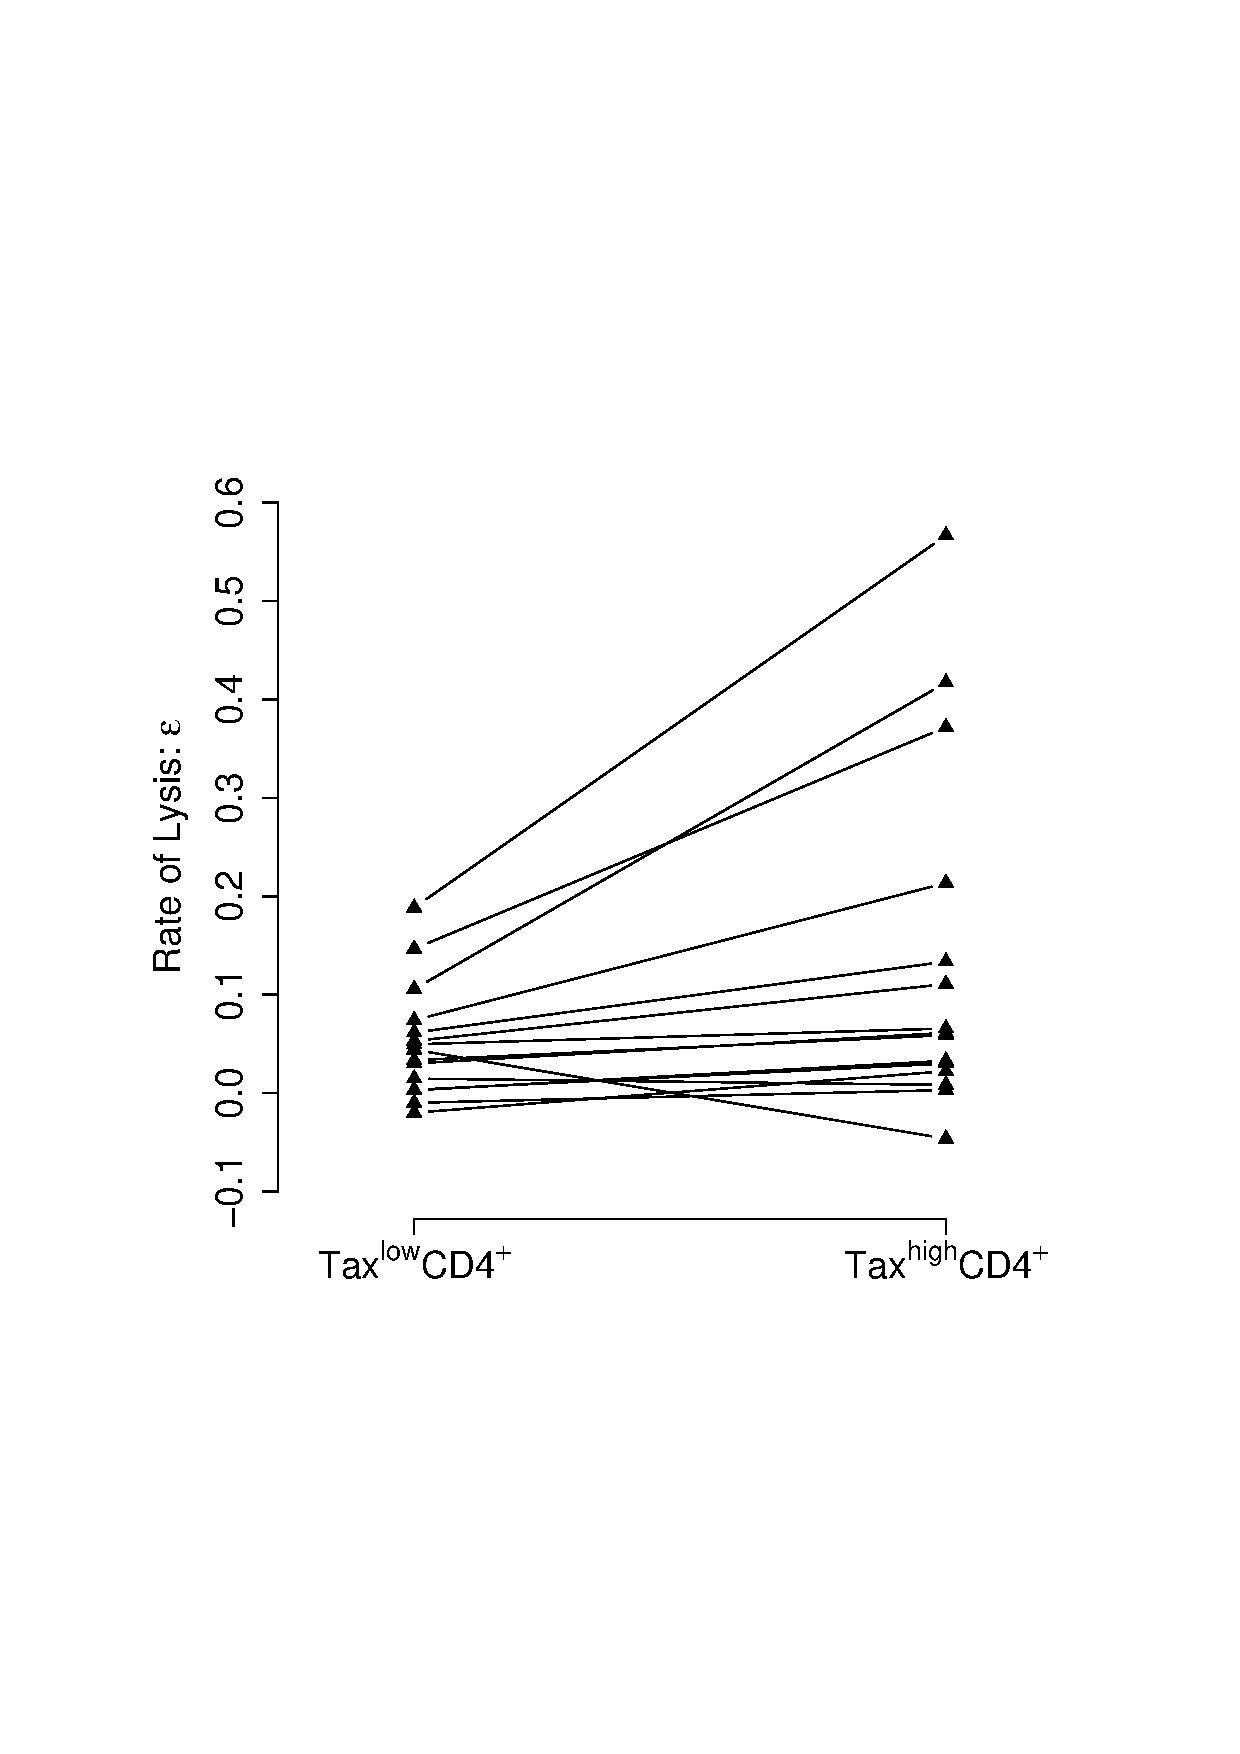
\includegraphics[width=14cm]{./Figures/chapter5/pairedEpsilon}
\caption[A paired comparison of the rates of lysis]{The rates of lysis $\epsilon$\superscript{low} and $\epsilon$\superscript{high} compared per patient. Tax\superscript{high} cells were killed faster than Tax\superscript{low} cells in the same individual ($P = 0.004$, Wilcoxon-Mann-Whitney, $n=15$).}
\label{chapter5/figurePairedEpsilon}
\end{figure}

\begin{figure}[htp]
\centering
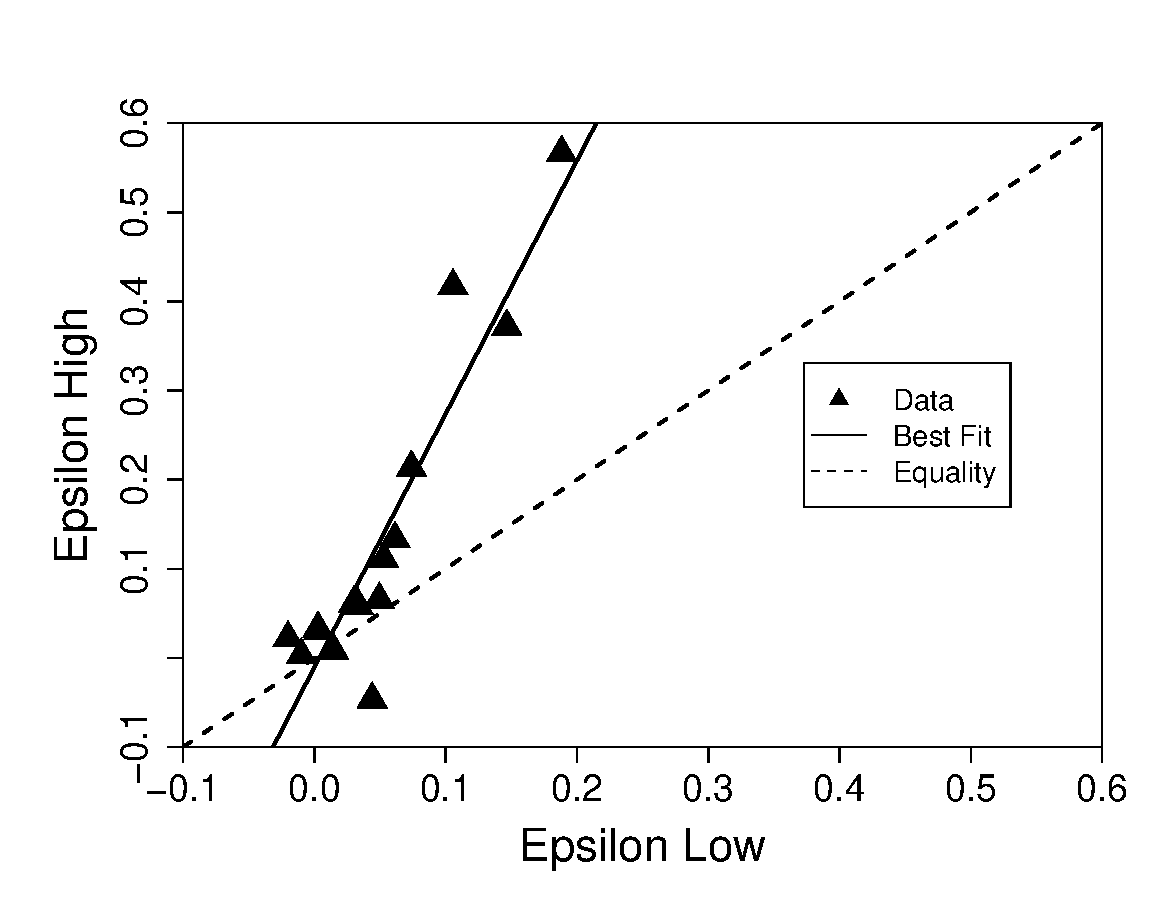
\includegraphics[width=14cm]{./Figures/chapter5/figureEpsilonHighLow}
\caption[The ratio of Tax\superscript{high}/Tax\superscript{high} lysis rates]{A comparison of the rates of lysis $\epsilon$\superscript{low} and $\epsilon$\superscript{high}. The data represents the average $\epsilon$\superscript{low} and $\epsilon$\superscript{high} from the 2 repeats per patient. The was a strong linear correlation across all patients for this ratio ($R^2 = 0.855$, $P < 0.001$).}
\label{chapter5/figureCompareLysis}
\end{figure}

\begin{table}[htp]
\begin{center}
{
\small
\begin{tabulary}{\textwidth}{|L|L|L|L|L|L|L|L|}
\hline
& Names & $C_1$ & $C_2$ & $\epsilon$ Low 1 & $\epsilon$ Low 2 & $\epsilon$ High 1 & $\epsilon$ High 2 \bigstrut \\
\hline
1 & HAP & 5.49168 & 0.80208 & 0.06325 & 0.03579 & 0.08192 & 0.04930 \bigstrut[t] \\
2 & HAY & 7.82112 & 0.34128 & 0.00998 & 0.01941 & -0.00819 & 0.02481 \\
3 & HBE & 8.55912 & 0.9036 & 0.10483 & 0.10640 & 0.41622 & 0.41790 \\
4 & HBX & 4.1112 & 0.29808 & 0.06160 & 0.06127 & 0.13806 & 0.12907 \\
6 & HCH & 6.78072 & 0.68136 & 0.07576 & 0.07223 & 0.24124 & 0.18569 \\
8 & HFB & 5.61096 & 0.9168 & -0.00280 & -0.01707 & -0.02105 & 0.02714 \\
11 & TAK & 4.80936 & 0.07488 & 0.03289 & 0.02731 & 0.05000 & 0.07240 \\
12 & TAQ & 3.87672 & 0.14112 & 0.03150 & 0.05664 & 0.04257 & -0.13534 \\
13 & TAW & 4.28592 & 0.86304 & 0.19241 & 0.18434 & 0.53716 & 0.59616 \\
14 & TAZ & 12.6408 & 0.27312 & 0.03840 & 0.02830 & 0.07164 & 0.04612 \\
15 & TBC & 53.83248 & 1.08096 & 0.00462 & 0.00097 & 0.03455 & 0.03117 \\
16 & TBJ & 14.04216 & 0.54552 & 0.15732 & 0.13589 & 0.42991 & 0.31358 \\
17 & TBP & 18.14064 & 0.87336 & -0.00313 & 0.00972 & 0.03025 & 0.02982 \\
19 & TCL & 2.9952 & 0.5952 & 0.05158 & 0.05430 & 0.11593 & 0.10564 \\
20 & UV1 & 2.5392 & 1.04928 & -0.02919 & -0.01079 & 0.04658 & -0.00212 \bigstrut[b] \\
\hline
\hline
& Names & $\epsilon$ Low Avg & $\epsilon$ High Avg & $\epsilon$ Low 1 SD & $\epsilon$ Low 2 SD & $\epsilon$ High 1 SD & $\epsilon$ High 2 SD \bigstrut \\
\hline
1 & HAP & 0.04952 & 0.06561 & 0.02272 & 0.02713 & 0.06017 & 0.02021 \bigstrut[t] \\
2 & HAY & 0.01469 & 0.00831 & 0.0178 & 0.02471 & 0.01251 & 0.04833 \\
3 & HBE & 0.10561 & 0.41706 & 0.0623 & 0.13736 & 0.30864 & 0.28325 \\
4 & HBX & 0.06143 & 0.13356 & 0.01437 & 0.0671 & 0.06328 & 0.12195 \\
6 & HCH & 0.07399 & 0.21347 & 0.0375 & 0.04678 & 0.18174 & 0.02042 \\
8 & HFB & -0.00993 & 0.00304 & 0.01811 & 0.02293 & 0.03427 & 0.04355 \\
11 & TAK & 0.0301 & 0.0612 & 0.01943 & 0.01747 & 0.05339 & 0.03249 \\
12 & TAQ & 0.04407 & -0.04639 & 0.01176 & 0.13824 & 0.05061 & 0.10499 \\
13 & TAW & 0.18837 & 0.56666 & 0.0659 & 0.07396 & 0.11129 & 0.32662 \\
14 & TAZ & 0.03335 & 0.05888 & 0.03852 & 0.0228 & 0.07298 & 0.04592 \\
15 & TBC & 0.0028 & 0.03286 & 0.0101 & 0.00806 & 0.02315 & 0.02376 \\
16 & TBJ & 0.1466 & 0.37175 & 0.04261 & 0.02233 & 0.19724 & 0.08156 \\
17 & TBP & 0.0033 & 0.03004 & 0.01462 & 0.00265 & 0.01026 & 0.0256 \\
19 & TCL & 0.05294 & 0.11078 & 0.09165 & 0.11836 & 0.13564 & 0.17345 \\
20 & UV1 & -0.01999 & 0.02223 & 0.0046 & 0.04018 & 0.11681 & 0.05295 \bigstrut[b] \\
\hline
\end{tabulary}
}
\end{center}
\caption[The summary statistics of the CTL lysis model]{The summary statistics for the model of CTL-mediated lysis efficiency against CD4$^+$ cells expressing either high or low levels of Tax. Each row gives the statistics per patient. The columns from left to right: $C_1$ and $C_2$ refer to the estimated rates of change per 24 hours between Tax\superscript{negative} and Tax\superscript{low} and Tax\superscript{low} and Tax\superscript{high} respectively. $\epsilon$ low 1 and 2 and $\epsilon$ high 1 and 2 give the values of $\epsilon$ derived from the model for the 2 repeats of low Tax and high Tax expressing cells respectively. $\epsilon$ low average and $\epsilon$ high average are the respective means of the 2 repeats. The next 4 columns show the standard deviation values derived from the estimates of $\epsilon$ for the 2 repeats of low and high. These were calculated using a bootstrap method (see \sref{chapter5/methodsBootstrap}).}
\label{chapter5/table1}
\end{table}


\begin{table}[htp]
\begin{center}
{
\small
\begin{tabulary}{\textwidth}{|L|L|L|L|L|L|L|L|}
\hline
 & Names & $R^2$ TC Low & $R^2$ TC High & $R^2$ High 1 & $R^2$ High 2 & $R^2$ Low 1 \bigstrut \\
\hline
1 & HAP & 0.45711 & 0.82968 & 0.76929 & 0.92048 & 0.86973 \bigstrut[t] \\
2 & HAY & 0.87095 & 0.84082 & 0.3946 & 0.29511 & 0.43637 \\
3 & HBE & 0.26648 & 0.49379 & 0.80528 & 0.93747 & 0.82434 \\
4 & HBX & 0.7376 & -1.49857 & 0.96126 & 0.78407 & 0.95216 \\
6 & HCH & 0.16752 & 0.43028 & 0.55425 & 0.97523 & 0.78886 \\
8 & HFB & -1.09248 & 0.77528 & 0.12536 & 0.39027 & 0.00464 \\
11 & TAK & 0.81652 & 0.46595 & 0.78497 & 0.95456 & 0.82724 \\
12 & TAQ & 0.94614 & 0.85412 & 0.8894 & 0.14617 & 0.913 \\
13 & TAW & -0.05858 & -0.21404 & 0.98371 & 0.89219 & 0.9684 \\
14 & TAZ & 0.84013 & 0.75042 & 0.64513 & 0.51961 & 0.46895 \\
15 & TBC & 0.61237 & 0.92676 & 0.87283 & 0.76828 & 0.089 \\
16 & TBJ & 0.75008 & 0.69859 & 0.86004 & 0.88222 & 0.72689 \\
17 & TBP & 0.73966 & 0.94565 & 0.94029 & 0.95061 & 0.06192 \\
19 & TCL & 0.63667 & 0.57808 & 0.89715 & 0.73001 & 0.64048 \\
20 & UV1 & -0.11191 & 0.67047 & 0.43589 & 0.00057 & 0.88353 \bigstrut[b] \\
\hline
\hline
 & Names & $R^2$ Low 2 &  $C$ Rep 1 & $C$ Rep 2 & $\epsilon$ Rep 1 & $\epsilon$ Rep 2 \bigstrut \\
\hline
1 & HAP & 0.47586 & 4.817 & 5.454 & 0.047 & 0.034 \bigstrut[t] \\
2 & HAY & 0.46641 & 8.705 & 9.021 & 0.008 & 0.021 \\
3 & HBE & 0.83602 & 6.585 & 13.191 & 0.081 & 0.2 \\
4 & HBX & 0.66433 & 4.552 & 4.294 & 0.077 & 0.067 \\
6 & HCH & 0.55311 & 4.052 & 4.09 & 0.037 & 0.032 \\
8 & HFB & 0.1863 & 3.106 & 3.617 & -0.015 & -0.002 \\
11 & TAK & 0.85024 & 5.798 & 5.664 & 0.04 & 0.035 \\
12 & TAQ & 0.51971 & 5.63 & 5.78 & 0.045 & 0.044 \\
13 & TAW & 0.92851 & 10.931 & 3.999 & 0.452 & 0.161 \\
14 & TAZ & 0.63307 & 14.711 & 12.33 & 0.044 & 0.027 \\
15 & TBC & 0.00652 & 51.142 & 52.394 & 0.013 & 0.01 \\
16 & TBJ & 0.83239 & 4.94 & 5.435 & 0.041 & 0.036 \\
17 & TBP & 0.87595 & 24.185 & 23.942 & 0.014 & 0.022 \\
19 & TCL & 0.75114 & 3.351 & 3.81 & 0.059 & 0.066 \\
20 & UV1 & 0.02592 & 2.216 & 1.988 & 0.008 & -0.004 \bigstrut[b] \\
\hline
\end{tabulary}
}
\end{center}
\contcaption{Continued: The $R^2$ values for fits of the model against the experimental data are shown for the time course model ($R^2$ TC low and $R^2$ TC high) and the 2 repeats in the lysis model ($R^2$ high and $R^2$ low). Finally the original values of the $C$ constant and $\epsilon$ are shown for 2 repeats per patient ($C$ Rep 1, $C$ Rep 2, $\epsilon$ Rep 1 and $\epsilon$ Rep 2).}
\end{table}

%%%%%%%%%%%%%%%%%%%%%%%%%%%%%%%%%%%%%%%%%%%%%%%%%%%%%%%%%%%%%%%%%%%%%%%%%%%%%%%%%%%%%%%%%%%%%%%%%%%%

\section{Discussion}

CD8$^+$ T cells have been shown in vitro to require only 10 complexes of MHC/peptide to elicit a lytic effector response \citep{Purbhoo2004, Sykulev1996, Christinck1991}. The detection of a significant difference in the rate of CTL-mediated lysis between cells with high Tax expression and those with low Tax expression was therefore surprising, since even the low Tax cells contain sufficient Tax protein to be readily detected by flow cytometry. Inefficient lysis might be caused by inefficient Ag processing, which would result in turn in few MHC/Tax peptide complexes being presented on the infected cell surface, despite the high level of intracellular Tax protein as indicated by intracellular staining. Alternatively, it is possible that there is not a uniformly high probability of CTL-mediated lysis when a low threshold of MHC/peptide density on the cell surface is exceeded, but rather that the probability of CTL-mediated lysis increases progressively with increasing density of MHC peptide complexes. Finally, it is possible that despite the immunogenicity of Tax protein in the CD8$^+$ T cell response \citep{Goon2004}, recognition of another HTLV-I Ag by CTLs might be the factor that limits the rate of HTLV-I replication in vivo \citep{Jacobson1990, Pique2000b}.